Os diagramas presentes nesta seção, detalham as configurações do servidor onde foram feitas as análises deste trabalho. 

\section{Rack do servidor utilizado para testes dos modelos de escalabilidade}

Foi utilizado durante todo trabalho o \textit{rack} Maritaca, que utiliza o sistema operacional Ubuntu 14.04 x86/64, com kernel 3.8.0-39-generic.

Conforme a Figura \ref{fig:maritaca-rack} e \ref{fig:real}, o \textit{rack} do servidor utilizado para as modelagens deste trabalho é composto por 9 \textit{nodes}, 2 \textit{header nodes}, 4 \textit{nobreaks} que alimentam as réguas de energia (\textit{power strip}), 2 \textit{switchs}, 1 teclado, 1 mouse e 1 monitor.

    \begin{figure}[htb]
    \centering
    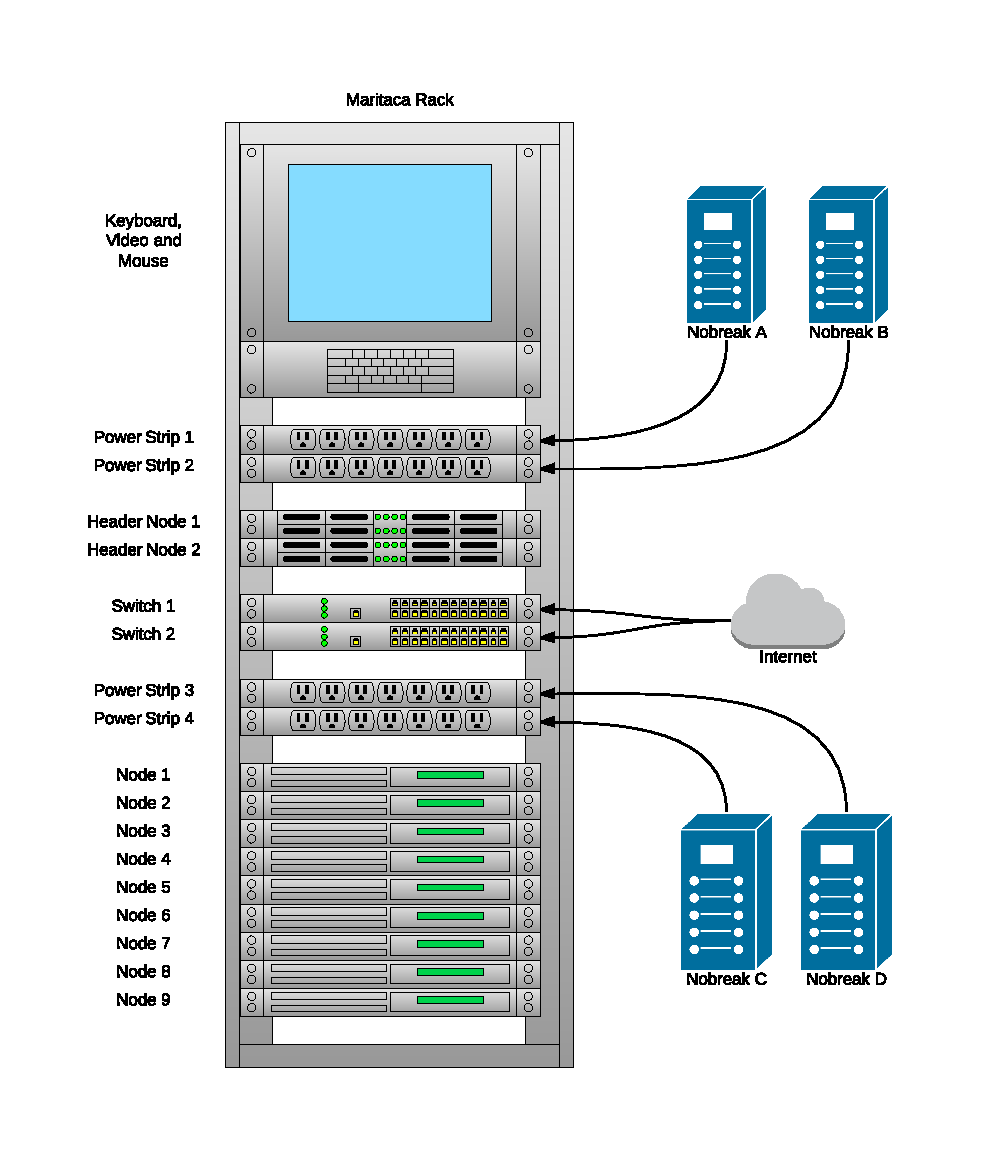
\includegraphics[scale=0.6]{imagens/maritaca-rack.pdf}
    \caption{\textit{Rack} do servidor Maritaca}
    \label{fig:maritaca-rack}
    \end{figure}

\begin{figure}[!htb]
\centering
\subfloat[Visão Frontal]{
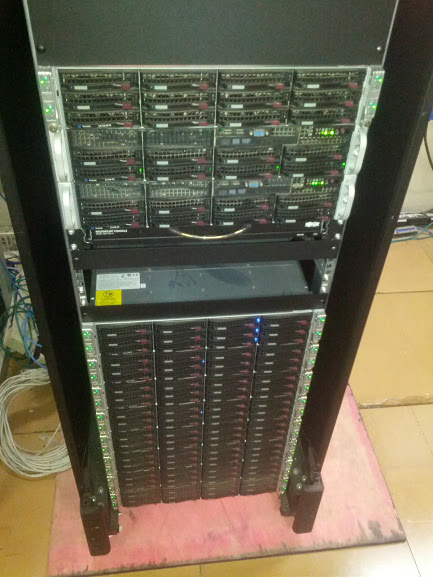
\includegraphics[height=7cm]{imagens/rack-frente.jpg}
\label{fig:frente}
}
\quad %espaco separador
\subfloat[Visão Traseira]{
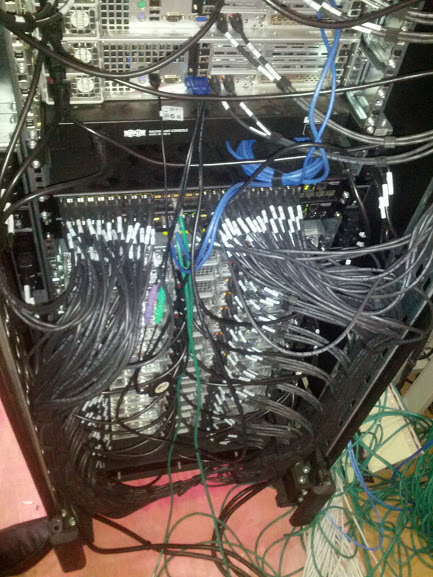
\includegraphics[height=7cm]{imagens/rack-tras.jpg}
\label{fig:tras}
}
\caption{Imagem real do \textit{rack} do servidor Maritaca}
\label{fig:real}
\end{figure}




\subsection{\textit{Nodes}}

Os \textit{nodes} possuem configurações de rede dinâmica enquanto no \textit{headnode} é estática. Apesar dos \textit{nodes} serem capazes de inicializar o sistema operacional, mesmo sem rede, o \textit{boot} nessas máquinas é controlado pelo \textit{headnode} que só permite a continuidade do \textit{boot} se toda a infraestrutura de rede necessária para virtualização e agregação remota de discos estiver satisfatória.

O \textit{rack} contém 9 \textit{nodes}, sendo que cada um possui 4 máquinas servidoras. Cada máquina destas é composta por 2 CPUs com a seguinte configuração: 

    \begin{itemize}
    
    \item Processador AMD Opteron (tm) 6344
    
        \begin{itemize}
        \item 12 \textit{cores};
        \item 200 MHz de \textit{clock};
        \item frequência de 2,6 GHz e
        \item 3 \textit{caches} com \textit{clock} de 1 GHz cada. Sendo que a primeira possui 576 kB de capacidade e as demais 12 MB.
        \end{itemize}
        
    \item 4 pentes de memória DDR3 \textit{synchronous}, sendo:
        
        \begin{itemize}
        \item 2 pentes com capacidade de 8 GB;
        \item 2 pentes com capacidade de 4 GB e
        \item ambos com 1,6 GHz de \textit{clock}.
        \end{itemize}

    \item 3 discos ATA \textit{Disk} com capacidade de 2 TB cada.

    \end{itemize}
    
    A Figura \ref{fig:node} exibe a frente de um \textit{node} e seus componentes de interface.
    
     \begin{figure}[htb]
    \centering
    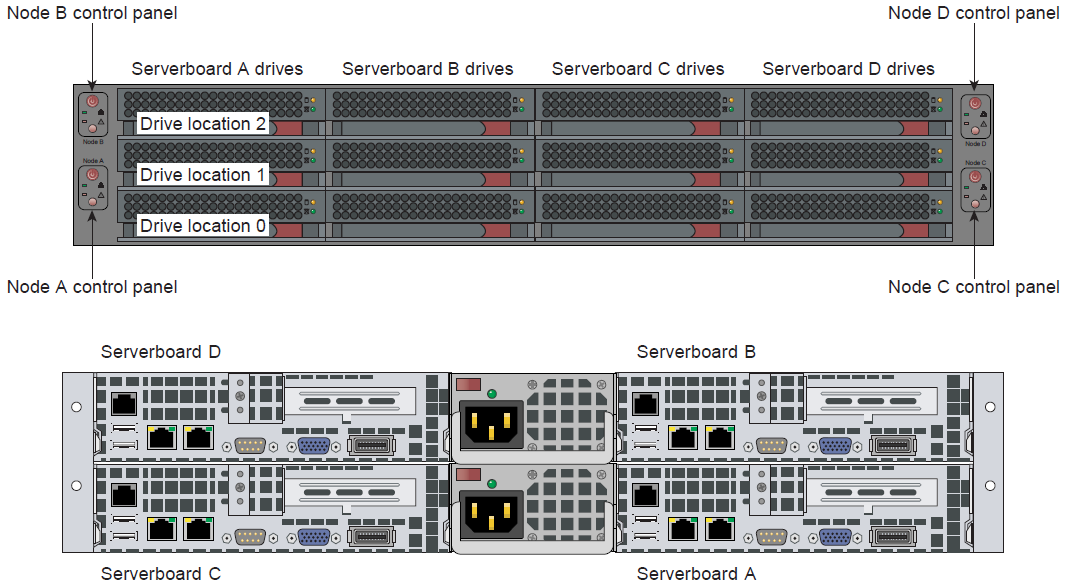
\includegraphics[scale=0.50]{imagens/node.png}
    \caption{Frente do \textit{node} e componentes de interface traseiros} \cite{SGI2011i}
    \label{fig:node}
    \end{figure}   
    
    
\subsection{\textit{Head Nodes}}

O \textit{head node} tem como função primária alojar todos os serviços necessários para o funcionamento dos \textit{nodes} que pertencem ao seu grupo principalmente as definições de rede, controle de \textit{boot} pxe, dhcp, dns interno, repositório interno para instalações automatizadas, \textit{midleware} de controle do \textit{cluster}.

    O \textit{rack} possui 2 \textit{head nodes}. Cada um possui 2 CPUs, estas por sua vez, possuem a seguinte configuração:

    \begin{itemize}
    
    \item Processador AMD Opteron (tm) 6344;
    
        \begin{itemize}
        \item 12 \textit{cores};
        \item 200 MHz de \textit{clock};
        \item frequência de 2,6 GHz e
        \item 3 \textit{caches} com \textit{clock} de 1 GHz cada. Sendo que a primeira possui 576 kB de capacidade e as demais 12 MB.
        \end{itemize}
        
    \item 4 pentes de memória DDR3 \textit{synchronous}, com capacidade de 8GB cada e 1,6 GHz de \textit{clock} em ambos;

    \item 2 discos ATA \textit{Disk} com capacidade de 2 TB cada;
    \item 1 DVD e 
    \item 2 PCI.

    \end{itemize}
    
A Figura \ref{fig:headnode} exibe a frente de um \textit{head node} e seus componentes de interface.

    \begin{figure}[htb]
    \centering
    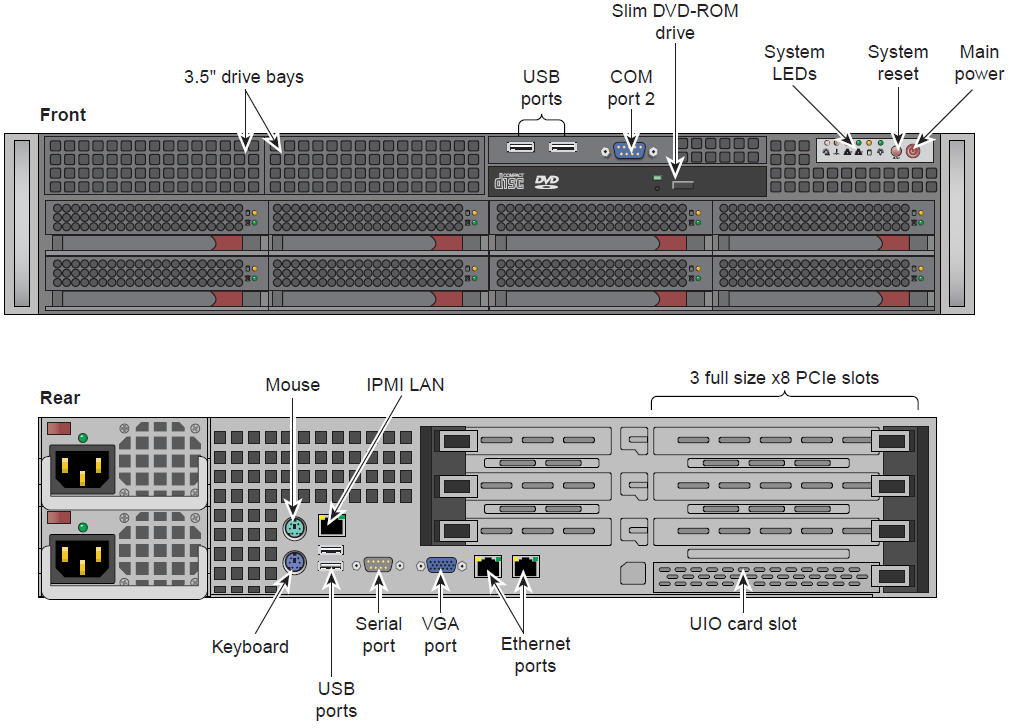
\includegraphics[scale=0.50]{imagens/headnode.png}
    \caption{Frente do \textit{head node} e componentes de interface traseiros} \cite{SGI2011}
    \label{fig:headnode}
    \end{figure}

\section{Redes virtuais e Redes Privadas}

    Em um sistema em computação em nuvem é extremamente importante isolarmos a rede dos \textit{hosts} da rede dos \textit{guests}. São redes que possuem funcionalidades diferentes e gerenciam pacotes de formas diferentes umas das outras.
    
    O isolamento de recursos garante que as redes virtuais operem de forma independente, assim, o uso de recursos de um roteador virtual não interfere no desempenho dos demais. O isolamento de recursos é importante porque evita a negação de serviços, já que uma rede virtual não consegue exaurir os recursos de outra rede virtual \cite{Carlos2011}.
    
    Na redes dos \textit{guests} são gerenciados pacotes de menores tamanhos, porém em maior quantidade. Pode-se citar como exemplo um servidor Tomcat, que responde a diversas requisições onde os pacotes possuem MTU $\leq$ 1500.
    Já na rede dos \textit{hosts}, existe outra infraestrutura de comunicação entre cada \textit{host}. Pode-se ter comunicações entre diferentes máquinas utilizando fibra óptica em placas de rede com transmissões em Gigabit.
    Neste tipo de rede, os \textit{hosts} se comunicam poucas vezes, porém os pacotes possuem MTU $\leq$ 9000, como ilustra a Figura \ref{fig:redesvirtpriv}.
    
    \begin{figure}[htb]
    \centering
    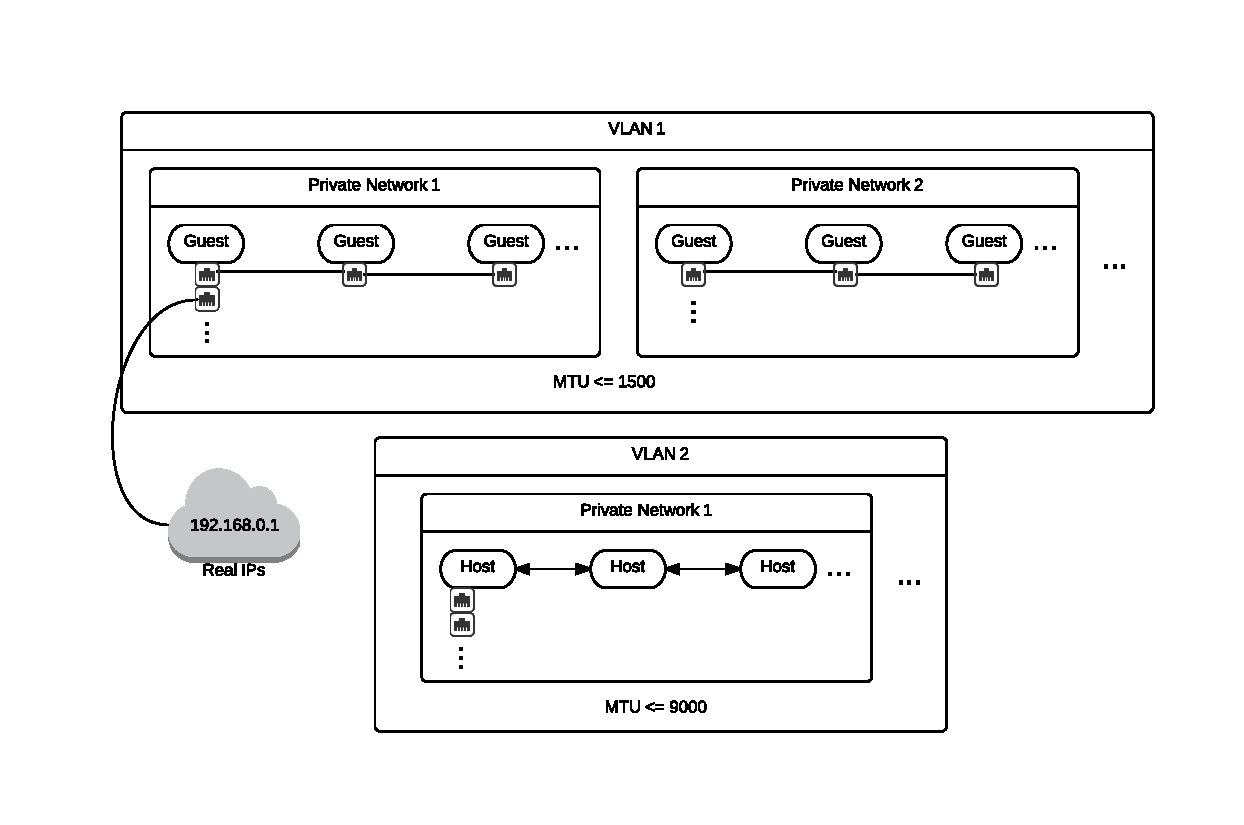
\includegraphics[scale=0.50]{imagens/esquema1.pdf}
    \caption{Diagrama das redes virtuais e redes privadas}
    \label{fig:redesvirtpriv}
    \end{figure}

\subsection{Isolamento das redes virtuais}

Como é necessário o isolamento entre as redes de \textit{hosts} e de \textit{guests}, as redes privadas dos guests são criadas dentro de uma VLAN e as redes privadas dos hosts são criadas dentro de outra VLAN.
A Figura \ref{fig:isolamento} ilustra o esquema de 2 VLANs, que podem ser descritas da seguinte forma:

    \begin{itemize}
        \item CORE: VLAN que abriga os serviços compartilhados como: DNS (\textit{private}), MySQL (\textit{cluster}), Load Balance (HAProxy), entre outros.
        \item GUESTs: VLAN que abriga as diversas redes privadas dos guests\footnote{Atualmente no servidor Maritaca, estão configuradas duas redes virtuais. A primeira é para atender os projeto Maritaca e a segunda (DIS) é destinada a atender outros projetos.}. Como cada guest é criado virtualmente, ele pode ter quantas interfaces de rede forem necessárias. As quais, por sua vez, podem ou não estar dentro de outras redes privadas pertencentes a esta ou outra VLAN.
    \end{itemize}

O \textit{Firewall} tem uma interface em cada rede, seja ela privada ou não. Ele também possui um IP real e é capaz de gerar um túnel da internet diretamente para as redes privadas. Utilizando o \textit{Firewall} também é possível criar conexões diretas entre as redes privadas. Porém, uma das principais desvantagens do seu uso para criação de conexões diretas é a utilização de NAT nestas conexões, pois NAT impossibilita o rastreio do caminho dos pacotes e aumenta o processamento dos dispositivos tradutores \cite{mattos}. 

    \begin{figure}[htb]
    \centering
    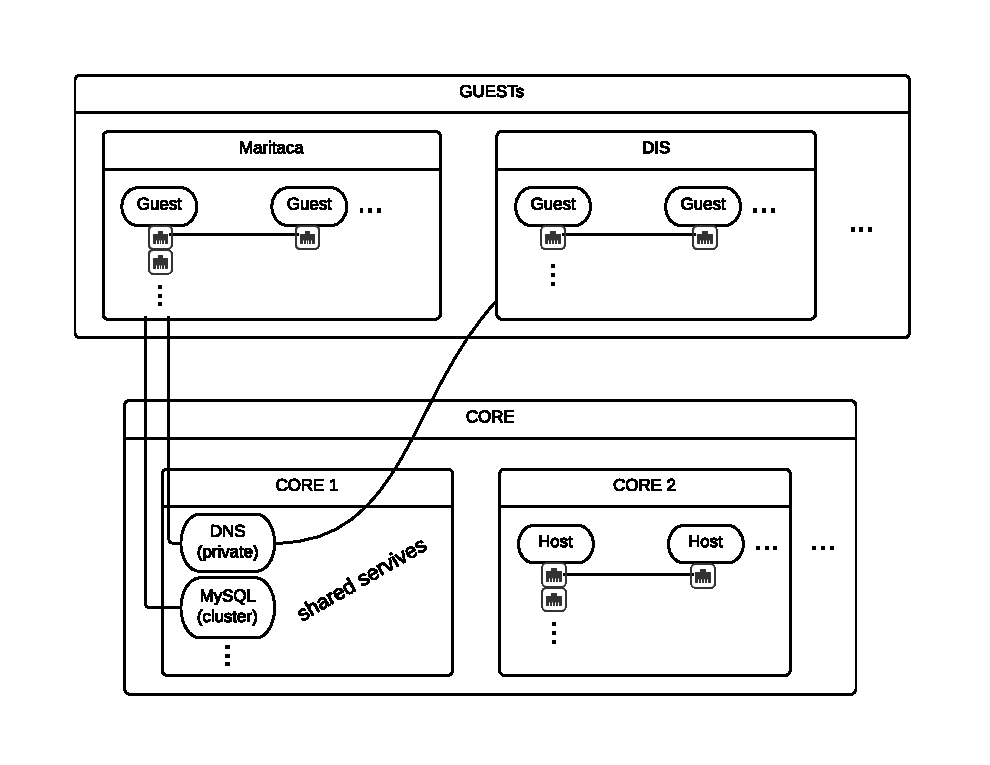
\includegraphics[scale=0.50]{imagens/esquema2.pdf}
    \caption{Isolamento das redes virtuais}
    \label{fig:isolamento}
    \end{figure}
    
\section{Balanceador de Carga (\textit{Load Balancer})}

O Balanceador de Carga recebe um pacote e direciona o mesmo ao servidor responsável pelo seu processamento.
Conforme a Figura \ref{fig:balanceador}, ele verifica a carga de cada servidor, para decidir qual servidor deverá receber aquele pacote.

    \begin{figure}[htb]
    \centering
    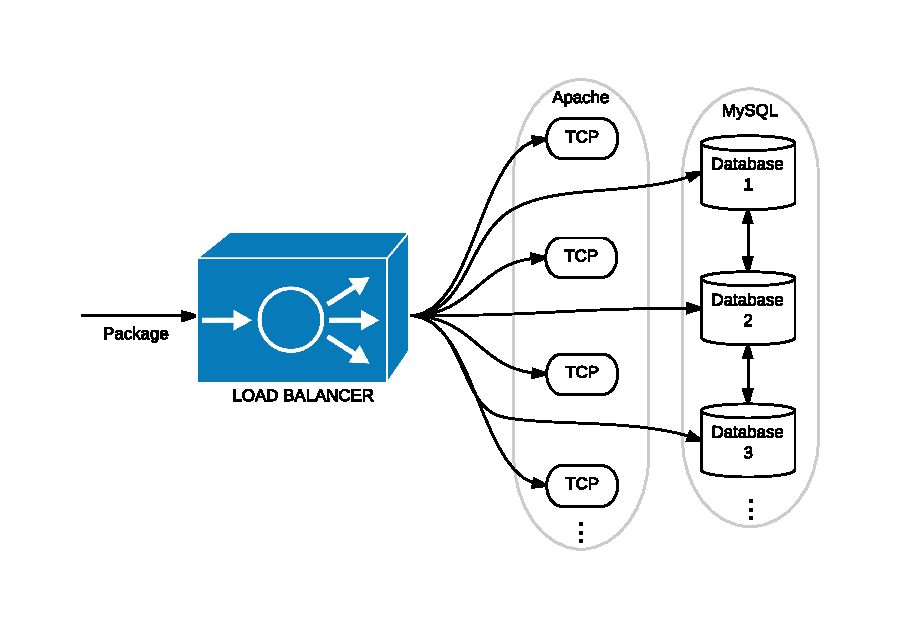
\includegraphics[scale=0.82]{imagens/esquema3.pdf}
    \caption{Esquemático do funcionamento do Balanceador de Carga}
    \label{fig:balanceador}
    \end{figure}    
    
    
\section{Integração do Balanceador de Carga às redes virtuais}
    Unindo os diagramas anteriores, temos o diagrama representado na Figura \ref{fig:integracaoloadbalan}, no qual pode-se perceber que o \textit{Load Balancer} funciona roteando pacotes para outros serviços do sistema. Além disso, o \textit{Load Balancer} pode também ser replicado de acordo com a necessidade, pois também se trata de um serviço configurado em \textit{guest}.
    
    \begin{figure}[htb]
    \centering
    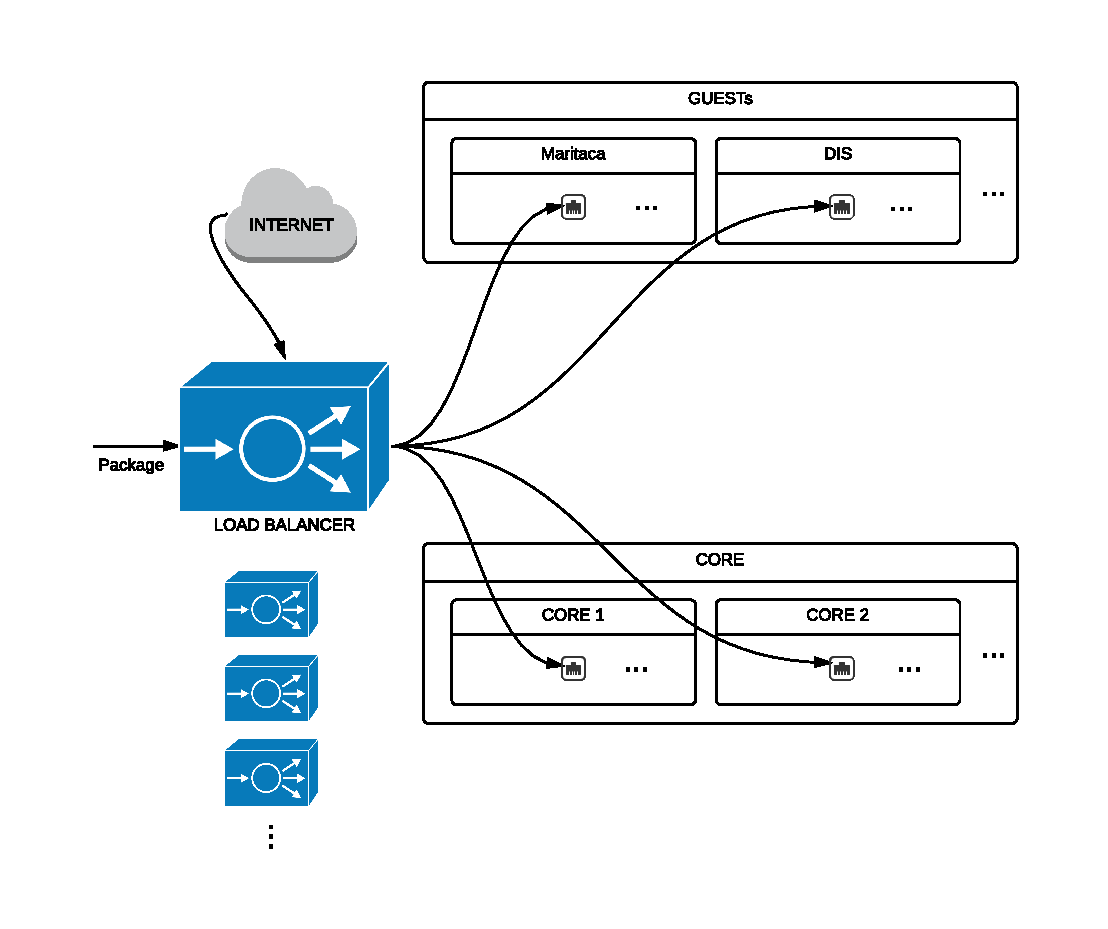
\includegraphics[scale=0.50]{imagens/esquema4.pdf}
    \caption{Integração do Balanceador de Carga às redes virtuais}
    \label{fig:integracaoloadbalan}
    \end{figure}


\section{Arquitetura do servidor}
Após a falha de um dos \textit{switches} as conexões das máquinas foram reorganizadas de forma que cada \textit{switch} atenda a um 1 \textit{headnode} e 18 \textit{nodes}. Com isso criou-se 2 grupos de máquinas denominados \textit{group1} e \textit{group2}. Esta reorganização foi necessária até que sejam adquiridos 2 cabos proprietários do fabricante do \textit{switch} capaz de conectar os \textit{switches} formando um pilha de única rede.

Os grupos de máquinas serão usados para virtualização sendo o \textit{group1} alocado para produção e \textit{group2} para testes de resiliência da infraestrutura, até que seja possível unificar os grupos. O \textit{group2} também poderá ser usado como \textit{failover} do \textit{group1} caso haja uma falha crítica de hardware, como houve com um dos \textit{switches}.

    \begin{figure}[htb]
    \centering
    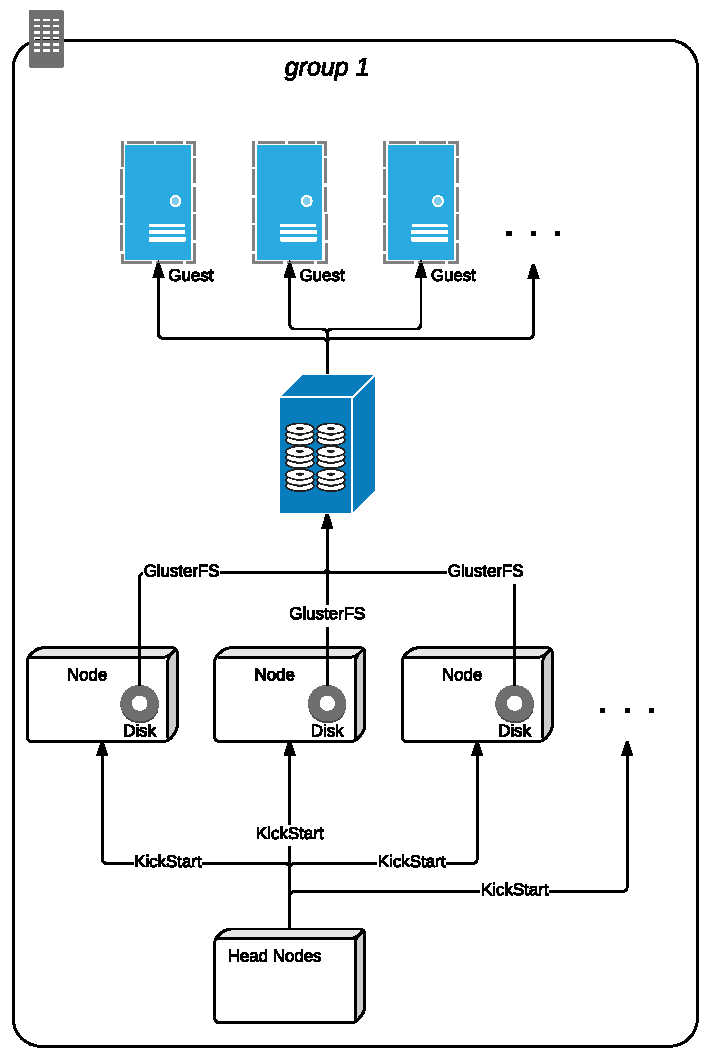
\includegraphics[scale=0.6]{imagens/group1.pdf}
    \caption{Arquitetura do \textit{group 1}}
    \label{fig:group1}
    \end{figure}

Atualmente o group1, representado na Figura \ref{fig:group1}, é composto pelo \textit{headnode}-1 e os \textit{nodes} de 32 à 20 mais o \textit{node} 18 totalizando 1 \textit{headnode} e 14 \textit{nodes}. Os 4 \textit{nodes} restantes estão alocados para o antigo grupo de trabalho do projeto Maritaca, que deverão ser incluídas no group1 assim que os serviços forem migrados para esta nova estrutura. Com 14 \textit{nodes} e 3 HDs de 2 Tb em cada foi configurado um disco virtual do tipo \textit{distributed replicated} com o glusterFS, no qual o volume replicado distribui os arquivos entre os \textit{bricks}, conforme a Figura \ref{fig:drv_gluster}. Este tipo de configuração é utilizada em servidores cuja exigência é a escala de armazenamento e a confiabilidade.  Com isso, o sistema de arquivos distribuído totaliza 38 Tb úteis para o alojamento dos discos virtuais das \textit{guests}.

    \begin{figure}[htb]
    \centering
    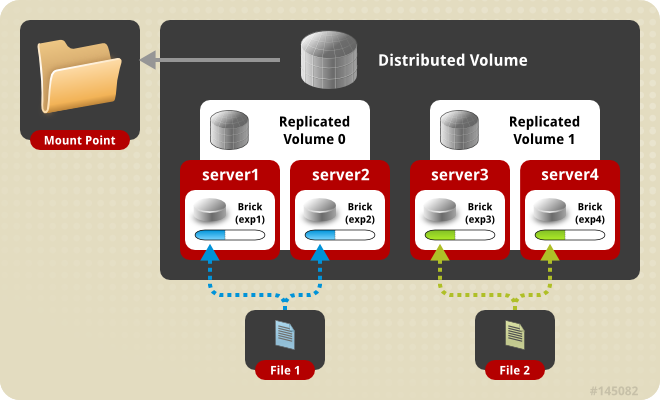
\includegraphics[scale=0.6]{imagens/Distributed_Replicated_Volume.png}
    \caption{Esquema de replicação distribuída via GlusterFS} \cite{Chandrashekar2015}
    \label{fig:drv_gluster}
    \end{figure}



Cada \textit{node} possui uma instalação Fedora Server 21 padronizada via Kickstart, sistema de arquivos distribuído via GlusterFS e camada de rede definida por software via OpenVSwitch.

Conforme a Figura \ref{fig:particoes}, a organização das partições dos \textit{nodes} pode ser vista pelo administrador executando o comando \textit{lsblk} no \textit{terminal}.

    \begin{figure}[htb]
    \centering
    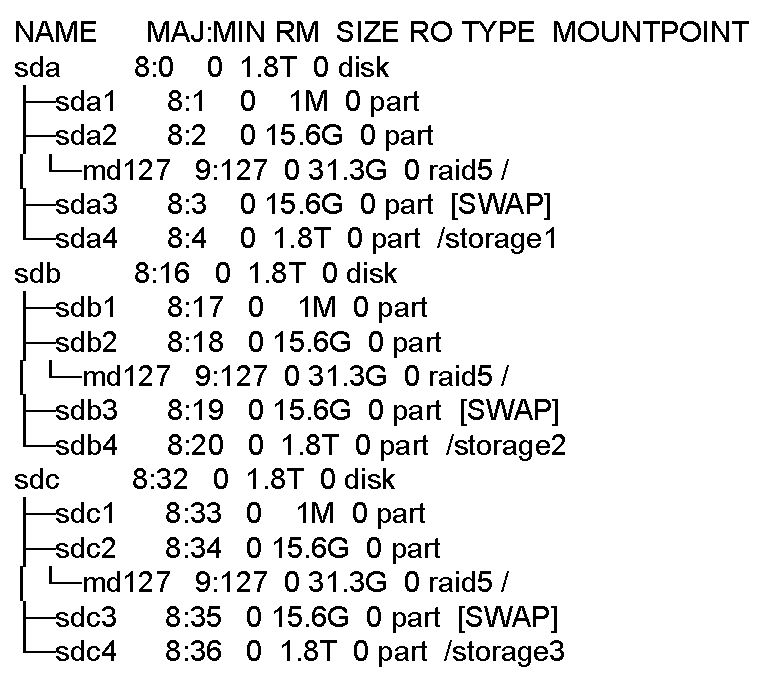
\includegraphics[scale=0.8]{imagens/particoes.pdf}
    \caption{\textit{Layout} de partições}
    \label{fig:particoes}
    \end{figure}

O \textit{layout} exibido na Figura \ref{fig:particoes}, é pré-resultado das linhas de automação, presentes no \textit{script} do Kickstart, que geram a instalação dos \textit{nodes}.
Neste \textit{layout}, o SO opera em um RAID5 que suporta a falha de um dos HDs. Os SWAPs estão distribuídos nos 3 HDs pois não são críticos para o funcionamento do sistema. A partição de \textit{boot} é replicada no ínicio de cada HD de forma que qualquer um deles contenha um setor inicializável (setor de \textit{boot}) para o RAID5 onde reside o SO. Cada HD possui uma partição de dados que será a base física para o volume GlusterFS (\textit{storage1, storage2 e storage3}). Cada \textit{storageX} é replicado via rede em outro \textit{storageX} residente em outro \textit{node} que não está na mesma lâmina. 



As \textit{guests} tem seus discos virtuais e suas configurações alojadas no volume GlusterFS. O libvirt de cada \textit{node} encarrega-se de virtualizar os recursos de CPU e memória para cada \textit{guest}. As \textit{guests} são capazes de migrar livremente entre os \textit{nodes} do group1 sem serem desligadas (\textit{livemigration}). A camada de rede necessária ao funcionamento das \textit{guests} é encapsulada na própria \textit{guest} na forma de uma abstração da camada de rede das \textit{hosts} definida e gerenciada pelo openVSwitch. A ligação entre as interfaces virtuais de rede das \textit{guests} com a rede física é feita através de VETH PAIRS ligadas às BRIDGES do openVSwitch. Estas conexões correm de forma virtualizada no kernel do SO dentro de NAMESPACES.

Conforme descrito na seção \ref{sec:gluster} o sistema de arquivos distribuídos GlusterFS agrega múltiplas unidades de armazenamento remotas em um único volume. As unidades de armazenamento (\textit{bricks}), são distribuídas pela rede em um único sistema de arquivos paralelo, permitindo uma escalabilidade de milhares de \textit{bricks} e vários petabytes de armazenamento. A Figura \ref{fig:vmfs} exibe os 42 \textit{bricks} que compõe o GlusterFS configurado no servidor Maritaca. 
    \begin{figure}[htb]
    \centering
    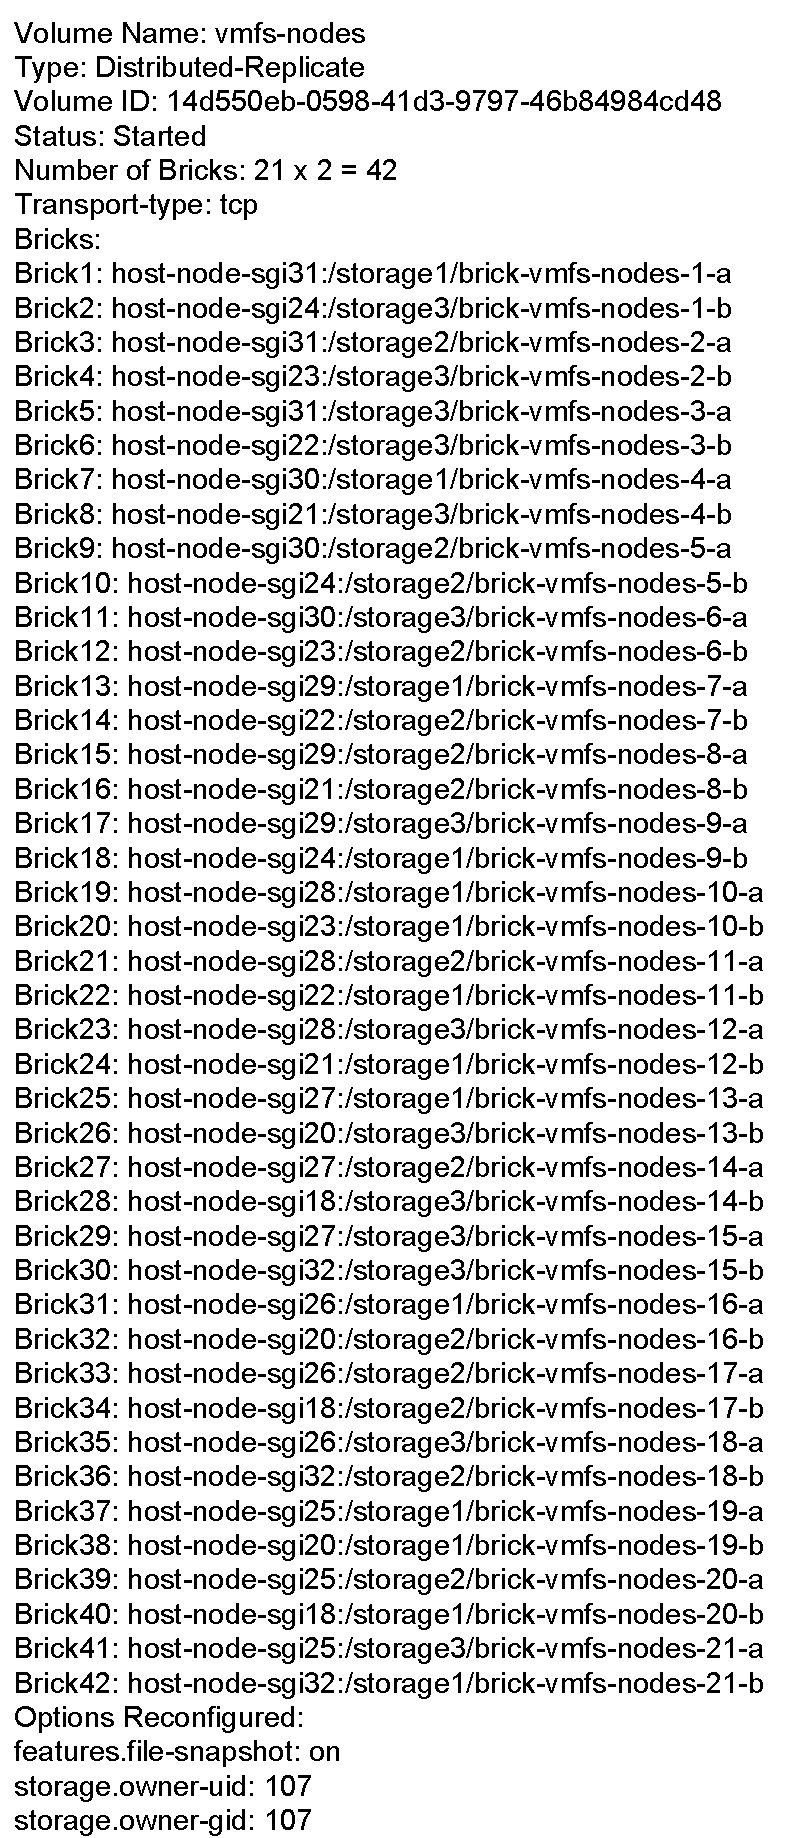
\includegraphics[scale=0.7]{imagens/vmfsnodes.pdf}
    \caption{\textit{Bricks} (GlusterFS)}
    \label{fig:vmfs}
    \end{figure}